%!TEX root= ../../../report.tex

\section{Model-based controllers}
\label{sec_dynamic_controller}
As introduced in the previous sections, the equations of motion derived for RuBi can be used to compute the necessary output values of its actuators in order to perform an input toes trajectory and external forces, as expressed in \ref{eq:tau_p}.
By definition, this could be sufficient to, appropriately used, be utilized as the base of a controller for the robot, without accounting the own dynamics of the actuators.
As an example of the above said, and despite the early stage in its development in which this model is left, some data has been computed and plotted for proving the concept.
The only trajectory planner current implemented computes vertical straight paths for the toes.
However, more complex trajectory equations could be used to achieve different locomotion patterns.

\begin{figure}[htb]
	\centering
	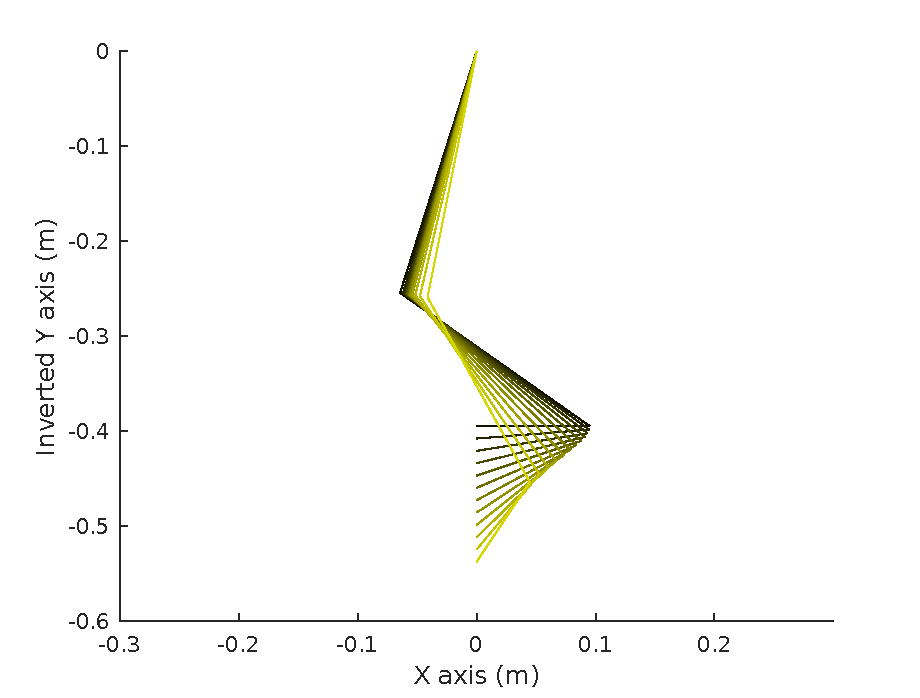
\includegraphics[width=0.5\textwidth]{figures/kinematics_sim.pdf}
	\caption{Joints trajectories from kinematics model.}
	\label{fig:controller_position}
\end{figure}

An initial and final toes position has been inputed to \ref{eq:toe_trajectory} to define an example trajectory for the toes in one leg, together with a random value for $\Delta h$.
The output of the kinematics computed for $i=1,...,N$ steps is shown in Figure \ref{fig:controller_position}, where it has been rearranged for visualization.
It can be seen that the toes trajectory does not cover the full range of a vertical jump.

\begin{equation}
\label{eq:joint_vel}
	\dot{\theta}_{i,j} =\frac{ \abs{ \theta_{j}(t_{i}) - \theta_{j}(t_{i-1}) } }{ t_{step} }
\end{equation}

For the trajectory described and $\Delta h$, the impulse equation in \ref{eq:impulse} has been computed and the values $(F_{min}, t_{max})$ from \ref{eq:work} have been used as input to the dynamic model.
The result of computing \ref{eq:dynamics_eq1} for the same time steps is shown in \ref{fig:controller_torque}, together with the solution for equation \ref{eq:joint_vel} in \ref{fig:controller_speed}, calculated in an analogue way.

\begin{figure}[htb]
    \centering
    \begin{subfigure}{0.49\textwidth}
        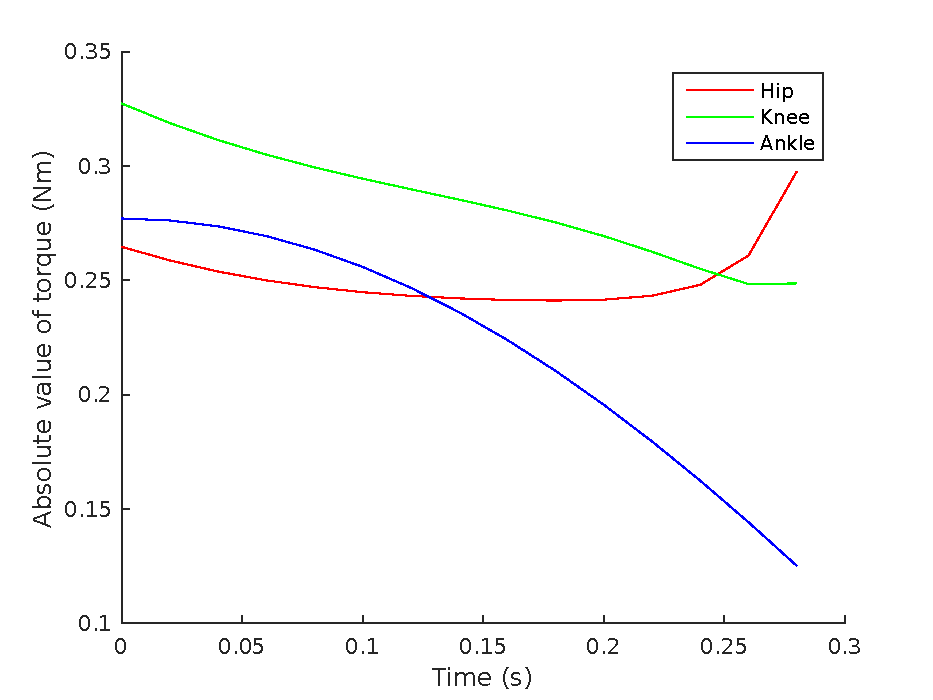
\includegraphics[width=\textwidth]{figures/torque-time.pdf}
		\caption{Joints torque as a function of time.}
		\label{fig:controller_torque}
	\end{subfigure}	
    \begin{subfigure}{0.49\textwidth}
        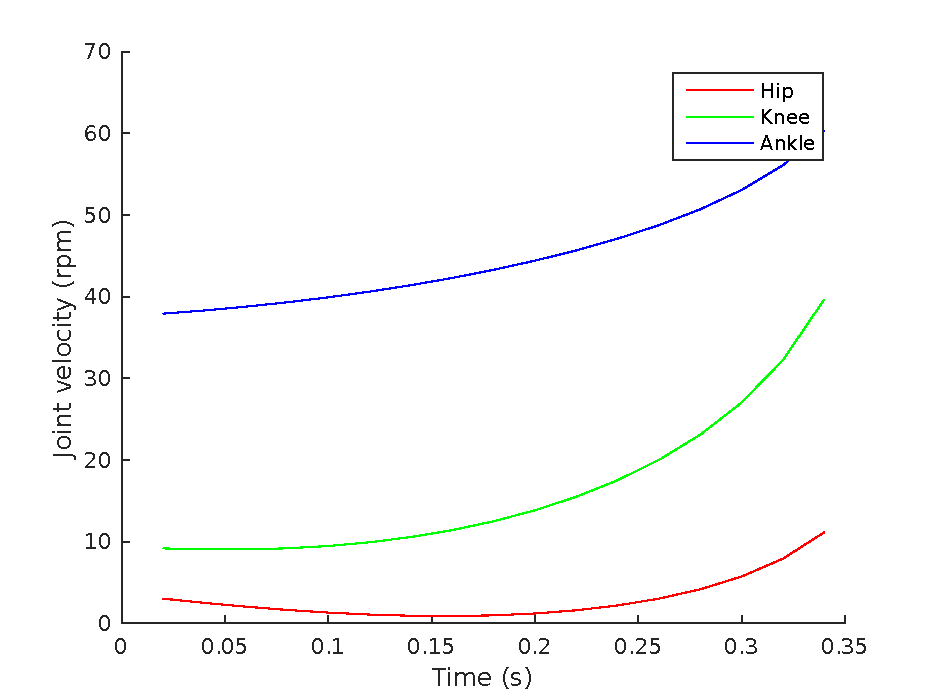
\includegraphics[width=\textwidth]{figures/speed-time.pdf}
		\caption{Joints velocity as a function of time.}
		\label{fig:controller_speed}
    \end{subfigure}
    \caption{Joint torque and velocity as a function of time.}
\end{figure}

The ranges in which the results in \ref{fig:controller_torque} and \ref{fig:controller_speed} are found seem consistent with the obtained during the experiments detailed in \ref{sub:suitability_of_the_motor_model_for_the_application}.
However, the analysis of their accuracy would entail a more precise construction of the mathematical model and study of kinematic chains dynamics which laid out of the scope of this project since it was not considered a priority goal.

